%\documentclass[prb,11pt,notitlepage]{revtex4-1}
%\documentclass[11pt,notitlepage]{revtex4-1}
\documentclass[11pt,a4paper]{article}
%---------------------------
% preambulo:
%---------------------------
\usepackage{abstract}
\usepackage[affil-it]{authblk}
\usepackage[utf8]{inputenc}	% encoding do arquivo, reconhecimento de acentos, etc.
\usepackage[brazilian]{babel}    % hiphenação em portugues
\usepackage{textcomp} % pacote para simbolos gregos no texto, sem ficar itálico
\usepackage{amsmath}    % need for subequations
\usepackage{amssymb}    % need for math symbols
\usepackage{graphicx}   % need for figures
\usepackage{verbatim}   % useful for program listings
\usepackage{color}      % use if color is used in text
\usepackage{subfigure}  % use for side-by-side figures
\usepackage{siunitx}
\usepackage{hyperref}   % use for hypertext links, including those to external documents and URLs
\usepackage[yyyymmdd,hhmmss]{datetime} % pacote para escrever a data de hoje
\usepackage[brazilian,nameinlink]{cleveref} % pacote para referenciar figuras e equacoes
\usepackage[table,xcdraw]{xcolor} % tabelas coloridas
\usepackage{circuitikz} %Pacote para desenhar circuitos
\usepackage{tikz}
\ctikzset{bipoles/length=0.9 cm} % tamanho dos componentes desenhados nos circuitos pelo pacote Circuitikz
\raggedbottom           % don't add extra vertical space
%---------------------------
%MARGENS
%---------------------------
\usepackage{indentfirst}        % indenta primeiro parágrafo
\setlength{\topmargin}{-15pt} % extra vert. space + at the top of header: 23pt
\setlength{\oddsidemargin}{-15pt} % extra spc added at the left of odd page: 0pt
\setlength{\textheight}{625pt} % comprimento do corpo do texto
\setlength{\textwidth}{480pt} % largura do corpo do texto
\setlength{\footskip}{50pt} % distancia da ultima linha de texto até número da pg.
%--------------------------
% INICIO DO DOCUMENTO:
%--------------------------
\begin{document}
%---------	
%cabeçalho
%---------
\title{Relatório 2: Resposta Temporal de Circuitos \\
\small{F429 - G.5  2$^{ \underbar{\text{o}} }$ semestre 2016 \\
Prof. Lázaro Padilha }}
\author{Giovani Nascimento Pereira - 168609 \\
Seong Eun Kim - 177143\\
Renan Adriani Sterle - 176536\\
Carlos Augusto Figueiredo Freire de Carvalho - 165684}
\affil{ Universidade Estadual de Campinas \\ Faculdade de Engenharia Elétrica e Computação \\ Campinas, SP}

\date{\today}

\maketitle
\begin{abstract}
    Nesse experimento, estudamos, na primeira parte, o funcionamento dos circuitos passa-alta e passa-baixa como diferenciadores e integradores, respectivamente, bem como o comportamento deles em diferentes faixas de frequência. Para isso, montamos circuitos RC e os analisamos quando submetidos a diferentes formas de onda de entrada e a variadas frequências. Dessa forma, pudemos calcular os valores da capacitância $((0.22 \pm 0.02) \mu F)$. Na segunda parte do experimento, estudamos o fenômeno do transiente em circuitos RLC e verificamos o papel do fator de qualidade na resposta temporal e a influência do resistor na constante de tempo de amortecimento e na frequência de relaxação. Para isso, montamos, circuitos RLC e observamos como muda a forma do transiente a diferentes resistências. Assim, pudemos analisar os estados de oscilação subamortecido, criticamente amortecido e superamortecido, e compreender melhor o efeito da resposta transiente e da solução permanente nos circuitos RLC.
\end{abstract}

\newpage % nova pagina
\tableofcontents % cria sumário

\newpage
\section{Introdução}
    
    O experimento 2 - Resposta Temporal de circuitos, foi realizado com o intuito de compreender melhor o funcionamento dos circuitos ressonantes RLC e de parte dos circuitos estudados, que foram Circuitos RC. Esse último tipo de circuito pode apresentar comportamentos interessantes como atuar como integrador ou diferenciador de funções de entrada em certas faixas de frequência. É uma extensão do estudo dos circuitos RC do Experimento 1 - Filtros, apenas focando em comportamentos mais específicos para certas faixas de frequência, e estudando melhor o comportamento em distintas situações.
    Da segunda parte do experimento, o principal objetivo era de observar e estudar melhor o funcionamento do circuito quando exposto a uma mudança abrupta (no caso, excitado por um degrau de tensão) para compreender a existência e relevância da resposta homogênea nos transientes dos circuitos. Esse tipo de comportamento é de importante compreensão pois se aproxima ou relaciona com outros sistemas reais (biológico, físico ou até mesmo financeiro) quando também quando ficam sujeitos à mudanças abruptas, e por isso o experimento pode dar uma base melhor para compreender esses fenômenos.
    
    % such introduction
    % much theory
    % very experiment
    % wow
    
\section{Objetivos}
    A primeira parte do experimento teve como objetivos estudar como o filtro RC pode atuar como integrador (passa-baixa) ou como diferenciador (passa-alta) do sinal de entrada, quando submetidos a bandas de freqüência para as quais ocorre atenuação. Investigamos, também, a aplicação das séres de Fourier para as formas de ondas utilizadas. Além disso, verificamos quantitativamente as relações de integração e diferenciação para sinais de entrada com onda senoidal, quadrada e uma cuja forma é a derivada de uma curva Lorentziana (“dLorentz”).
    
    A segunda parte teve como objetivo estudar o comportamento dos circuitos RLC em situações de amortecimento. Mais especificamente, o fenômeno do transiente nesse tipo de circuito e investigar a influência da resistência na constante de tempo de amortecimento e na freqüência de relaxação do circuito e o significado do fator de qualidade (Q) na resposta temporal dos circuitos.
    
    
\section{Metodologia}

    \subsection{Parte A - Circuitos Integradores e Diferenciadores}
    
    Na primeira parte do experimento, foram estudados os circuitos RC integradores e diferenciadores, conforme descritos na \cref{CircIntegDif}.
    
    \begin{figure}[ht] %ht tenta colocar a figura aqui ("here") e se  não der, colocar no topo ("top") da página
    \centering
    %FIG. 1A
    \subfigure[Filtro passa-baixas]{
    \begin{circuitikz}[european][scale=1]
    	\node (Xi) at (0.7,0.7) {$V_1$};
    	\node (Xf) at (3.7,0.7) {$V_2$};
    	\draw [semithick,->] (Xi) -- (0.1,0.1);
    	\draw [semithick,->] (Xf) -- (3.1,0.1);
    	\draw to [generic, o-o, l_=$R$] ++(2,0)
    		(2,0) to [short,o-o] ++(1,0)
    		(2,0) to [generic, o-o, l=$C$] ++(0,-2)
    		node[ground] {};
    \end{circuitikz}
    }
    %FIG. 1B
    \subfigure[Filtro passa-altas]{
    \begin{circuitikz}[scale=1]
    	\node (Xi) at (0.7,0.7) {$V_1$};
    	\node (Xf) at (3.7,0.7) {$V_2$};
    	\draw [semithick,->] (Xi) -- (0.1,0.1);
    	\draw [semithick,->] (Xf) -- (3.1,0.1);
    	\draw to [generic, o-o, l_=$C$] ++(2,0)
    		(2,0) to [short,o-o] ++(1,0)
    		(2,0) to [generic, o-o, l=$R$] ++(0,-2)
    		node[ground] {};
    \end{circuitikz}
    }
        \caption{\textbf{Circuitos integrador e diferenciador utilizando circuitos RC}}
    \label{CircIntegDif} %identificador da figura, usado para referência
    \end{figure}

    Para tanto, foi utilizada uma \textit{Protoboard} para auxiliar na montagem do circuito, e permitir que fosse desmontado e alterado facilmente, um osciloscópio e um gerador de função, ligados a um computador e conectados ao \texttt{MatLAB}, para a aquisiçao de dados.
    
    De ambos os circuitos pode-se derivar a seguinte expressão através das leis de Kirchoff:
    
    \begin{equation}
        R\dfrac {dq\left( t\right) }{dt}+\dfrac {q\left( t\right) }{C}=V_{1}\left( t\right)
    \label{eq:1}
    \end{equation}
    
    A \cref{eq:1} representa a equação de estado do circuito (EDO de primeira ordem) e da corrente em função do tempo.
    
    Desses circuitos é possívelo definir a \textit{frequência de corte} ($f_0$) que representa um limitante que serpara comportamentos muito distintos do circuito para $f << f_0$ e $f >> f_0$.
    
    \begin{equation}
        f_0 = \dfrac{1}{2 \pi RC}
    \label{f0}
    \end{equation}
    
    
    No circuito passa-baixa, a frequências altas ($f >> f_0$), podemos considerar que a corrente que atravessa o circuito é quase nula, e  a variação temporal do sinal é muito rápida, de forma que não há tempo para as cargas se acumularem nos terminais do capacitor. Assim, podemos desprezar a queda de tensão no capacitor decorrente da lei de Kirchoff ($\dfrac {q\left( t\right) }{C}$). Fazendo isso, obtemos a expressão:
    
    \begin{equation}
        V_{2}\left( t\right) =\dfrac {q\left( t\right) }{c}=\dfrac {1}{c}\int i\left( t'\right) dt'
    \label{eq:2}
    \end{equation}
    
    
    Para o circuito passa-altas, uma expressão equivalente pode ser obtida a partir da \cref{eq:1}. Temos que para o circuito da \cref{CircIntegDif}a a tensão $V_2$ equivale a:
    
    $V_{2}\left(t\right)=Ri=R\dfrac{dq}{dt}$
    
    Mas $\dfrac{dq}{dt}$ é desprezível quando a frequência é muito baixa, $f<<f_0$, pois como o circuito é passa-alta, a corrente é quase nula. Assim:
    
    $V_{1}\left( t\right) =\dfrac {q\left( t\right) }{c}\Rightarrow q\left( t\right) =C\cdot V_{1}\left( t\right)$
    
    Então, podemos escrever a expressão de $V_2$ como:
    
    $V_{2}\left( t\right) =R\dfrac {d\left( CV_{1}\left( t\right) \right) }{dt}=RC\dfrac {dV_{1}\left( t\right) }{dt}$
    
    Dessa forma, no circuito passa-alta, o sinal é dado por:
    
    \begin{equation}
        V_{2}\left( t\right) \simeq RC\dfrac {dV_{1}\left( t\right) }{dt}
    \label{eq:3}
    \end{equation}
    
    %%Expa - item 4
    Depois, usando cada um dos circuitos da \cref{CircIntegDif}, o gerador de função foi ligado na forma de onda quadrada com tensão de pico-a-pico $V_{pp}=1$.
    O osciloscópio foi ligado ao circuito utilizando-se os dois canais medindo a forma de onda em $V_1$ e $V_2$.
    Então, a frequência do gerador foi variada de 100Hz a 100KHz, e as formas de onda geradas observadas com o auxílio do osciloscópio.
    %%Expa - item 5
    Após essas observações a forma de onda foi ajustada para a forma senoidal, ainda mantendo a tensão de pico-a-pico em $V_{pp}=1$. Com o osciloscópio ainda ligado ao circuito e obtendo as formas de onda, foi variado o \textit{offset} do gerador de função e os resultados observados através do osciloscópio.
    
    %%Expa - Item 6
    %%Expa - item 7
    %%Expa - Item8
    Após todas as observações, para cada um dos circuitos da \cref{CircIntegDif}, foram capturadas com o uso de um script no \texttt{MatLAB} as formas de onda referentes ao comportamento dos circuitos para frequências baixas, próximas e altas em relação à frequência de corte de cada um, e usando três formas de onda diferentes geradas pelo gerador de função: senoidal, onda quadrada e \textit{dlorentz}.
    
    Quando a função de entrada é da forma senoidal, é possível expressar as ondas na forma de fasores, facilitando a integração e diferenciação.
    
    \begin{equation}
        F(t) = f exp(j\omega t)
    \label{ID}
    \end{equation}
    
    Manipulando o fasor representado na \cref{ID} é possível obter para o circuito RC Passa-alta:
    
    \begin{equation}
        H_{p}.a.\left( \omega \right) =\dfrac {R}{R-jx_{c}}=\dfrac {1}{1-j\left( wRC\right) }\Rightarrow \{ ^{jwRC=RCH_{d}\omega,\quad \omega << 1/RC}_{1,\qquad \qquad \qquad \omega >> 1/RC}
        \label{PA}
    \end{equation}
    
    Analogamente, para o circuito RC integrador, ou, passa-baixa:
    \begin{equation}
        V_2=-jC_c/R-jX_c= \dfrac{\dfrac{-j}{\omega RC}}{1-\dfrac{j}{\omega RC}}\Rightarrow \{ ^{j/wRC,\qquad \qquad \omega >> 1/RC}_{1,\qquad \qquad \qquad \omega << 1/RC}
        \label{PB}
    \end{equation}
    
    \subsection{Parte B - Transientes em circuitos RLC}
    
    %%Expb - Item 1
    Na segunda parte do experimento (parte b), a fim de estudar o fenômeno do transiente nos circuitos RLC, foi montado na \textit{Protoboard} o circuito da \cref{CircResson}a. Para isso, foi usado uma resistência de década com $R=100\Omega$, um capacitor de $C=0,22\mu$F e um indutor de $L=48,42mH$. Então, o circuito foi ligado ao gerador de função com a forma de onda senoidal e o osciloscópio foi conectado com $V_1$ e $V_2$ na forma XY. Utilizando o refinamento de frequência do gerador de função, a frequência de entrada, \textit{$f_0$}, foi alterada até que a imagem observada no osciloscópio fosse uma reta diagonal (a 45\textdegree  de inclinação com a horizontal), o que  representava o estado ressonante do circuito, ou seja, que a tensão aplicada e a medida estavam totalmente fora de fase.
    
    
        \begin{figure}[!htb]
        \centering
        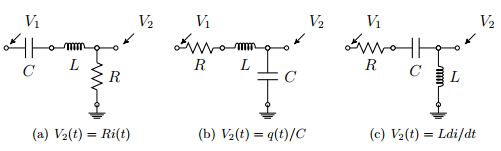
\includegraphics[scale=0.7]{CircResson.png}
        \caption{Montgem de Circuitos Ressonantes RLC com marcação da expressão de medição da tensão em $V_2$}
        \label{CircResson}
        \end{figure}
    
    A lei de Kirchoff para os circuitos da \cref{CircResson} é:
    
    \begin{equation}
        L\dfrac{d^{2}q\left(t\right)}{dt^{2}}+R\dfrac{dq\left(t\right)}{dt}+\dfrac{q\left(t\right)}{C}=V_{1}\left(t\right)
    \label{eq:4}
    \end{equation}
    
    A solução dessa EDO é composta de duas partes, a solução homogênea e a solução particular. O comportamento da solução homogênea tem um caráter de decaimento exponencial e, dessa forma, só é perceptível em períodos próximos aos transientes, enquanto em períodos mais longos, ela é imperceptível.
    
    Para melhor compreensão, podemos reescrever a \cref{eq:4}, dividindo-a por L e definindo algumas constantes novas:
    
    \begin{equation}
        \dfrac {d^{2}q\left( t\right) }{dt^{2}}+2\gamma \dfrac {dq\left( t\right) }{dt}t+\omega ^{2}_{0}q\left( t\right) =\dfrac {V_{1}\left( t\right) }{L}
    \label{eq:5}
    \end{equation}
    
    Onde $\omega _0=1/\sqrt{LC}$ é a frequência angular natural de oscilação do circuito, e $\gamma=R/2L$ é a taxa de amortecimento do sistema.
    
    Podemos definir o fator de qualidade (Q) como sendo:
    
    \begin{equation}
        Q=\dfrac {\omega _0}{\delta \omega} = \dfrac{\omega _0}{ 2 \gamma}
    \label{eq:6}
    \end{equation}
    
    Disso, podemos depreender que:
    \begin{itemize}
        \item Caso $\gamma< \omega _0$, ou seja, $Q>1/2$:\\
        O sistema é subamortecido.
        \item Caso $\omega _0 = \gamma$, ou seja, $Q=1/2$:\\
        O sistema é criticamente amortecido
        \item Caso $\gamma> \omega _0$, ou seja, $Q<1/2$:\\
        O sistema é superamortecido.
    \end{itemize}
    
    Resolvendo a \cref{eq:5}, a solucão homogênea é:
    
    \begin{equation}
        %%Solucao homogenea
        q_h\left(t\right)=e^{-\gamma t}\left(q_1 e^{-j\omega t}+q_2 e^{j\omega t}\right)
    \label{eq:7}
    \end{equation}
    
    Pode-se notar que a solução decai exponencialmente, conforme descrito acima, por isso o transiente caracteriza um fenômeno momentâneo.
    
    É possível inferir que a solução particular da \cref{eq:4} é uma constante no caso em que estudamos, em que para $t<0$, $V_1 =0$; e para $t>0$, $V_2>0$ e constante (função degrau). Assim a solução da EDO pode ser descrita como:
    
    \begin{equation}
        %%Solucao homogenea
        q_h\left(t\right)=CV_1 + e^{-\gamma t}\left(q_1 e^{-j\omega t}+q_2 e^{j\omega t}\right)
    \label{eq:8}
    \end{equation}
    
    Onde $CV_1$ corresponde a solução particular da EDO.
    
    %%Expb - Item 4
    Depois, com o circuito da \cref{CircuitoTriplo}a e calculado $f_0$, o gerador de função foi alterado para a forma de onda quadrada com a tensão pico-a-pico $V_{pp}=2V$, mas dessa vez com um período grande da onda a fim de observar a resposta transiente ao degrau de tensão. 
    
    Ajustando a imagem no osciloscópio foi possível observar o comportamento da tensão de saída em comparação à de entrada ($V_1$ e $V_2$, respectivamente) no degrau do transiente, \cref{TransOscilo}. O comportamento da tensão de saída é semelhante ao de um oscilador amortecido. Ao manter-se o valor da resistência de década pequeno (na ordem de 100$\Omega$), o sistema apresentou um comportamento oscilatório. Isso ocorre porque a resistência R do circuito funciona como um dissipador de energia num sistema oscilatório e, variando-se esse valor, altera-se o comportamento observado no osciloscópio.
    
    
    %%Expb - Item6
    Depois, o valor de R da resistência de década foi variado a fim de observar os casos de sub-amortecimento, em que era possível observar a oscilação da tensão de saída; de amortecimento crítico, quando a tensão para de oscilar no transiente; e de super-amortecido, para valores de R acima do do caso sub-amortecido.


    Assim que foram observadas as pequenas oscilações mostradas pelo osciloscópio, conforme pode ser observado na \cref{TransOscilo}a, foi feita uma montagem a fim de investigar melhor este comportamento.
    O circuito da \cref{CircResson}a foi montado novamente e dessa vez, o valor da resistência de década foi ajustado para se equivaler ao valor da queda de tensão interna do gerador de função. Nessa caso, a forma de onda obtida no canal de $V_2$ deveria ser idêntica a observada no canal da tensão de entrada, $V_1$. Depois, foi utilizada a função de soma do osciloscópio, e no caso $R_D=R_i$, onde $R_i$ é a resistência interna do gerador de função, a curva vermelha obtida da soma das duas deveria representar exatamente a forma de onda do transiente para a onda quadrada, como pode ser observado na \cref{SomaQuadrada}.
    
    Por fim, os 3 circuitos da figura \cref{CircResson} foram montados separadamente, e com o auxílio do \texttt{MatLAB} e de equipamentos ligados ao computador, foram obtidas as formas de onda geradas por cada circuito para o estado sub-amortecido de ressonância. As imagens estão dispostas na \cref{CircuitoTriplo}.
    
    

\newpage
\section{Resultados}
    
    %%Expa - Resultados da parte A do experimento
    \subsection{Resposta temporal dos circuitos Integrador e Diferenciador}
    
    As formas de ondas obtidas na parte A do experimento foram:
        \begin{figure}[!htb]
        \centering
        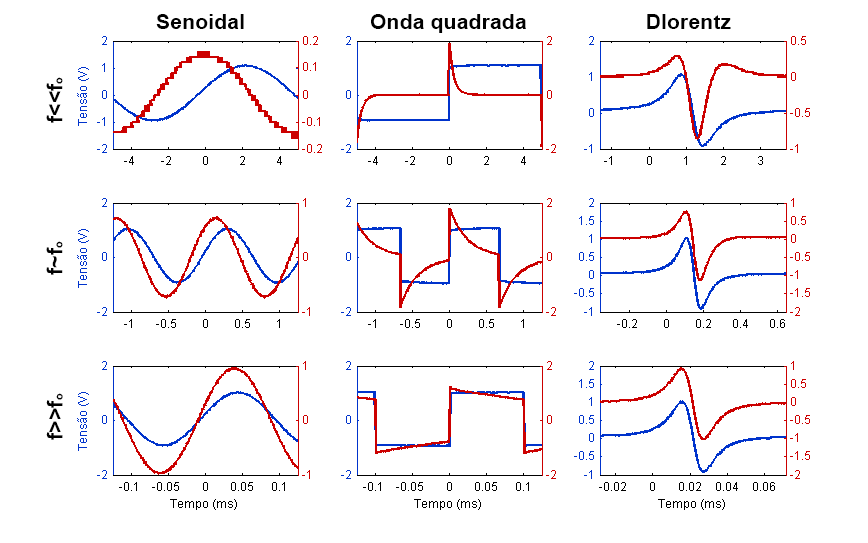
\includegraphics[scale=0.8]{PassaAltaVarredura.png}
        \caption{Formas de onda obtidas da varredura do circuito passa-altas (circuito diferenciador) da \cref{CircIntegDif}a. As colunas representam a forma de onda utilizada na entrada do circuito sendo senoidal, quadrada e \textit{dlorentz} respectivamente. E as linhas estão a mesma frequência da fonte sendo: baixa frequência, frequência próxima à frequência de corte e altas frequências, respectivamente}
        \label{PassaAltaVarredura}
        \end{figure}
    
    
        \begin{figure}[!htb]
        \centering
        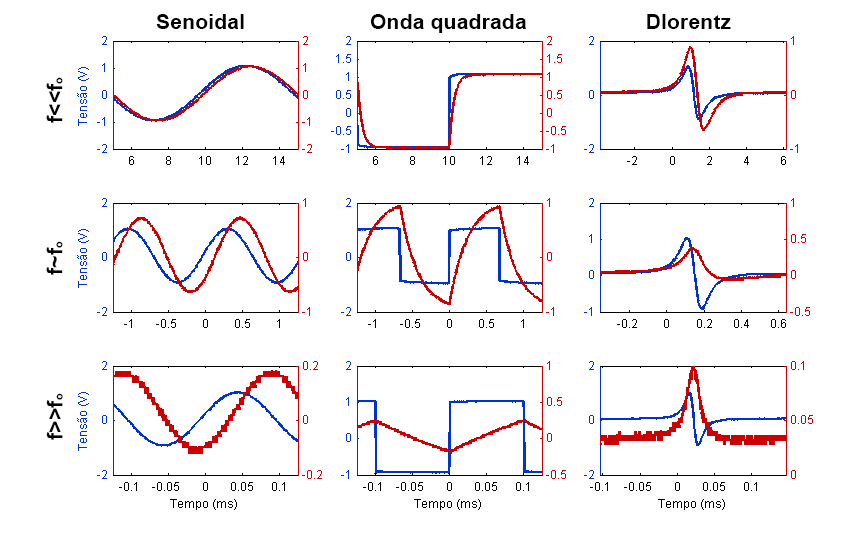
\includegraphics[scale=0.8]{PassaBaixaVarredura.png}
        \caption{Formas de onda obtidas da varredura do circuito passa-baixas (circuito integrador) da \cref{CircIntegDif}b. As colunas representam a forma de onda utilizada na entrada do circuito sendo senoidal, quadrada e \textit{dlorentz} respectivamente. E as linhas estão à mesma frequência da fonte sendo: baixa frequência, frequência próxima à frequência de corte e altas frequências, respectivamente}
        \label{PassaBaixaVarredura}
        \end{figure}
        
    \newpage
    \subsection{Transientes em circuitos RLC}
    Para a parte B do experimento, o comportamento da tensão de saída em comparação à de entrada ($V_1$ e $V_2$, respectivamente) no degrau do transiente, está representada na \cref{TransOscilo}.
    
        \begin{figure}[!htb]
        \centering
        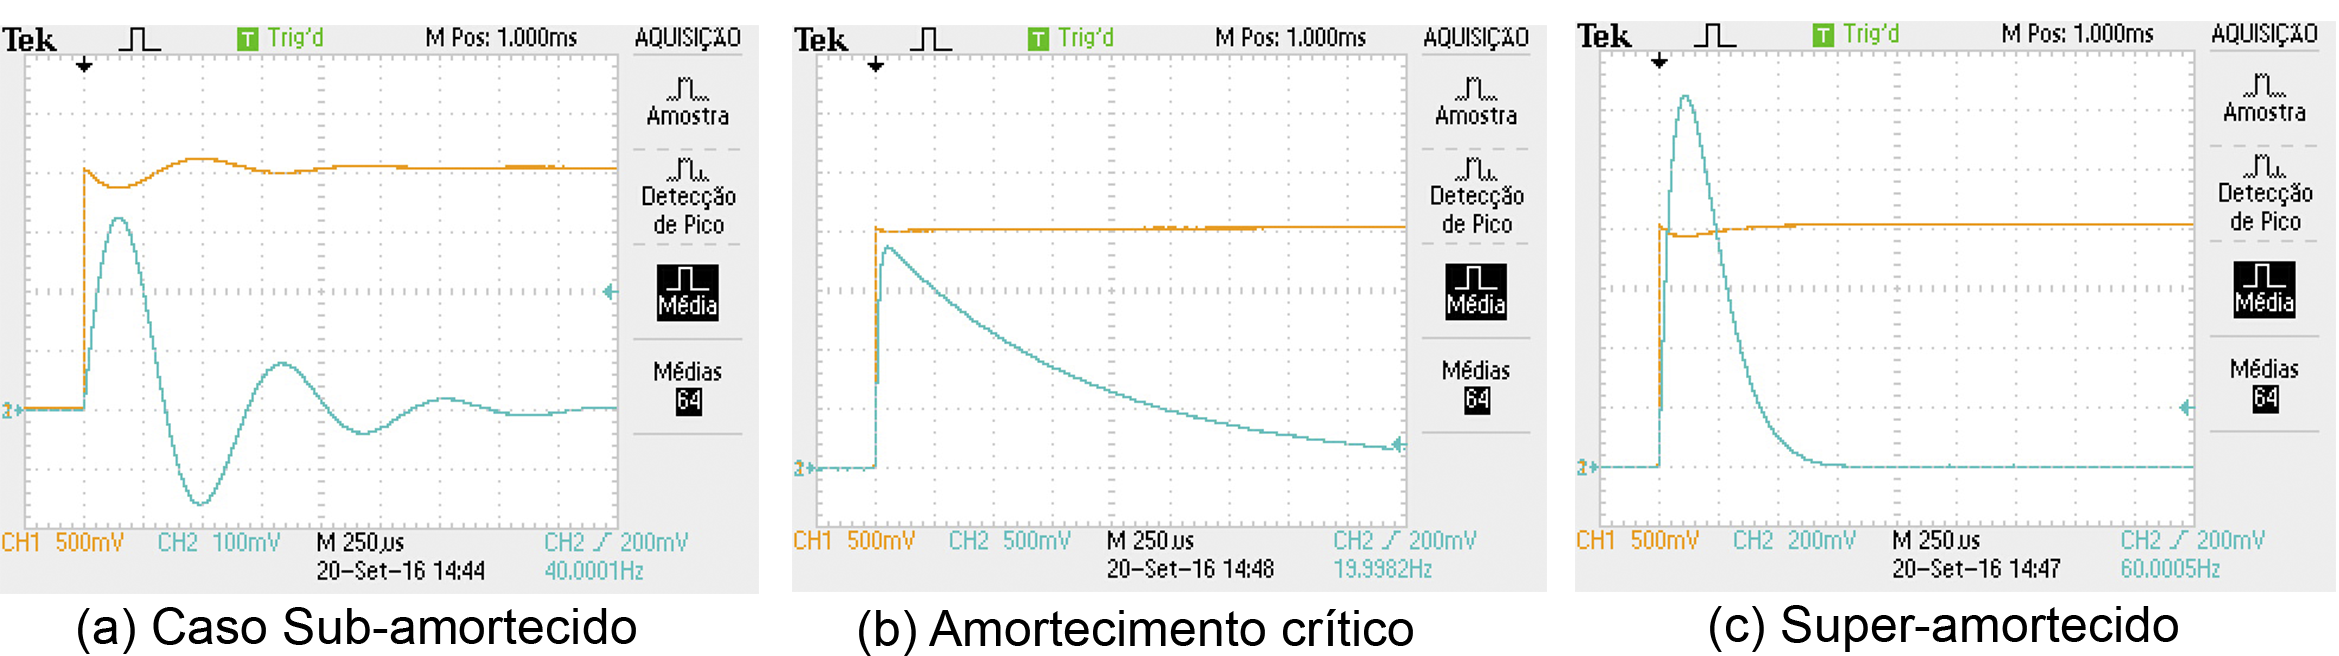
\includegraphics[scale=0.55]{TransienteOsciloscopio.png}
        \caption{Imagens obtidas pelo osciloscópio para os três casos de amortecimento. As informações dispostas ao longo das imagens foram geradas automaticamente pelo osciloscópio.}
        \label{TransOscilo}
        \end{figure}
        
    Ao montarmos o circuito da \cref{CircResson}a novamente e, ajustado o valor da resistência de década, as formas de ondas obtidas estão representadas na \cref{SomaQuadrada}.
    
        \begin{figure}[!htb]
        \centering
        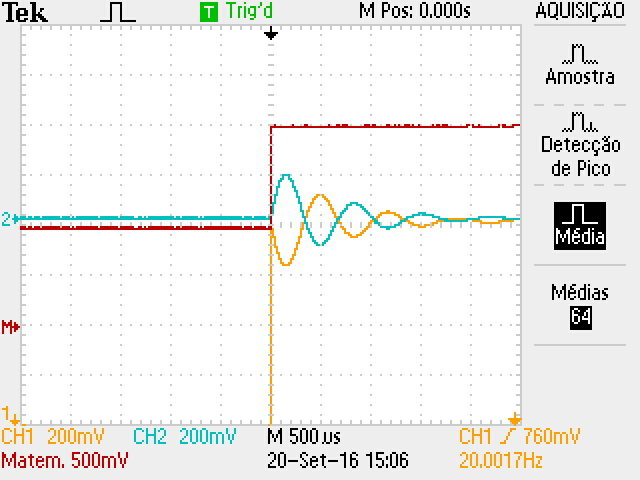
\includegraphics[scale=0.75]{SomaQuadrada.JPG}
        \caption{Imagens obtidas pelo osciloscópio das formas de onda de $V_1$ e $V_2$ e da soma das duas ondas. As formas de onda dos canais 1 e 2 estão deslocadas entre si, para facilitar a visualização do fato que são ondas complementares (estão exatamente fora de fase). As informações dispostas ao longo da imagem foram geradas automaticamente pelo osciloscópio.}
        \label{SomaQuadrada}
        \end{figure}
        
    Por fim, as formas de ondas obtidas quando os 3 circuitos da \cref{CircResson} estavam no estado sub-amortecido de ressonância estão representados na \cref{CircuitoTriplo}.
    
        \begin{figure}[!htb]
        \centering
        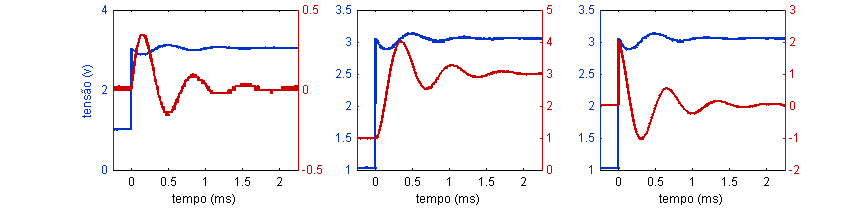
\includegraphics[scale=0.8]{CircuitoTriplo.png}
        \caption{Imagens obtidas pelo osciloscópio do estado de oscilação para o sistema sub-amortecido para os três circuitos da \cref{CircResson}, respectivamente.}
        \label{CircuitoTriplo}
        \end{figure}

\newpage
\section{Análise de Dados}

    \subsection{Circuitos Integradores e Diferenciadores}

    Através dos dados obtidos das varreduras digitais, dispostos em \cref{PassaAltaVarredura} e \cref{PassaBaixaVarredura}, pode-se fazer algumas análises. Para a montagem dos circuitos, de acordo com a \cref{CircIntegDif}, foi utilizado resistência de $R=100K\Omega$, pois esse valor de resistência é muito mais alto que a resistência interna do gerador de função (que é da ordem de $100\Omega$), isso garante que a queda de tensão na resistência interna do gerador seja pequena o suficiente para não causar distorções na forma de onda medida no canal 1.
    
    A frequência de corte dos circuitos, $f_o$, pode ser calculada através da \cref{f0} como:
    
    $f_{0}=\dfrac{1}{2\pi{RC}}=(74 \pm 7)10Hz$
    
    Como nos circuitos foram utilizados $R=(968\pm 1)\Omega$ e $C=(0.22\pm 0.02)\mu F$.
    
    Esse valor de f é uma frequência que divide o comportamento do circuito. Ele é diferente para frequências próximas de $f_0$, muito menores e muito mais altas que ele.
    
    Para o circuito da \cref{CircIntegDif}b, que é o passa-baixa (possível integrador), temos o comportamento observado em \cref{PassaBaixaVarredura}. A \cref{eq:2} prevê que a altas frequências, o circuito atua como integrador da tensão de entrada. Podemos notar que na linha de baixas frequências (gráficos da primeira linha), a tensão de entrada é aproximadamente a mesma de saída, isso se deve pois circuitos passa-baixa, para frequências muito menores que a de corte, permitem a passagem quase total da tensão pelo circuito. 
    
    Já na segunda linha de gráficos, em que a frequência é próxima da frequência de corte, o comportamento do circuito muda, e já é possível observar parte do comportamento integrador do circuito, pois apresentam uma significativa diferença de fase, e a tensão de saída é menor do que a de entrada. Além disso, observa-se que a primeira forma de onda é uma senoide, tanto na entrada, quanto na saída.
    
    E na última linha da figura, o circuito também demonstra comportamento integrador. Como o circuito é um passa-baixa, ele retém a passagem de tensões a altas frequências. Mas agora é possível observar o comportamento integrador do circuito. No caso da primeira figura, a senoide, a integral de uma função senoide é uma função de mesma forma, mas defasada em 1/4 de período, ou seja, com diferença de fase $\phi =\frac {-\pi} {2} rad$.
    Através da função de medição do osciloscópio foi possível obter que a diferença de fase entre as duas ondas era de $\phi =$($-89.20 \pm 0.01$$)^o$.
    
    Esse valor de diferença de fase é bem próximo de $\frac{-\pi}{2} rad$ ($-90^o$), que é o valor esperado, então é possível notar que o circuito estava atuando como um integrador da função de entrada.
    
    Agora, ao variar o \textit{offset} da entrada nesse circuito, como se trata de um circuito integrador, foi possível observar a onda do canal 1 ($V_1$) se deslocar no sentido vertical, e a onda do canal 2 ($V_2$) sofreu um crescimento constante, correspondente à integração da componente DC da entrada.
    
    Usando ainda a banda em que o circuito está integrando, $f>>f_0$, e tendo medido os valores de $V_1$ e $V_2$ nessa situação, é possível utilizar esses dados para encontrar a capacitância total C do circuito.
    
    $V_{1pp}=(1.04 \pm 0.02)V$, $V_{2pp}=(40 \pm 20)mV$
    
    $\mid H \mid = \mid V_{2pp}/V_{1pp} \mid = 1/\omega RC$
    
    $C = \mid V_{1pp}/V_{2pp} \mid 1/\omega R$
    
    $C = 0.21 \pm 0.02 \mu F$
    
    A capacitância encontrada está dentro do valor esperado, que é o valor nominal do capacitor utilizado ($C_0 = (0.22 \pm 0.02 \mu F)$).
    
    Agora, para o circuito da \cref{CircIntegDif}a, o passa-alta, diferenciador, o comportamento do circuito está descrito na \cref{PassaAltaVarredura}. A \cref{eq:3} prevê que o comportamento do circuito, para baixas frequências, é de um diferenciador e, para frequências altas, toda tensão de entrada no circuito é transmitida para a tensão de saída.
    
    Na \cref{PassaAltaVarredura}, podemos notar que na primeira linha de gráficos, que estão com a entrada a baixas frequências, o circuito atua como um diferenciador da função de entrada. Podemos concluir isso pois a primeira forma de onda é senoidal, e a derivada de uma senoide é uma senoide defasada em $\pi /2$, como representado. A segunda forma de onda é uma onda quadrada, e a tensão de saída apresenta um comportamento interessante, como nos \textit{vales} e \textit{cristas}, onde a tensão é uma constante, a tensão de saída é nula, pois a derivada de uma constante é nula. Isso muda apenas nos transientes, quando a derivada assume um valor alto, mas logo volta para zero pelo fato de a entrada se tornar constante novamente. E a derivada da função \textit{Dlorentz} também pode ser observada na última figura.
    
    Na segunda linha da imagem, onde as frequências são próximas da frequência de corte, pode-se notar uma visível mudança no comportamento do circuito. E na última linha, onde $f >> f_0$, A tensão medida em $V_1$ é praticamente a mesma medida em $V_2$, já que o circuito se trata de um passa-alta.
    
    Nesse mesmo circuito, variando-se o \textit{offset}, foi possível visualizar um deslocamento em $V_1$, mas não em $V_2$, isso porque a entrada do \textit{offset} representa uma constante na função de entrada, e o circuito atua como um diferenciador, e a derivada de constantes é nula.
    
    Podemos observar melhor o caso da curva Dlorentz para compreender o comportamento integratório e diferenciador dos circuitos observados anteriormente. A \cref{Dlorentz}, mostra esse comportamento.

    %%ADICIONAR ITEM 6 DA PARTE A
        \begin{figure}[!htb]
        \centering
        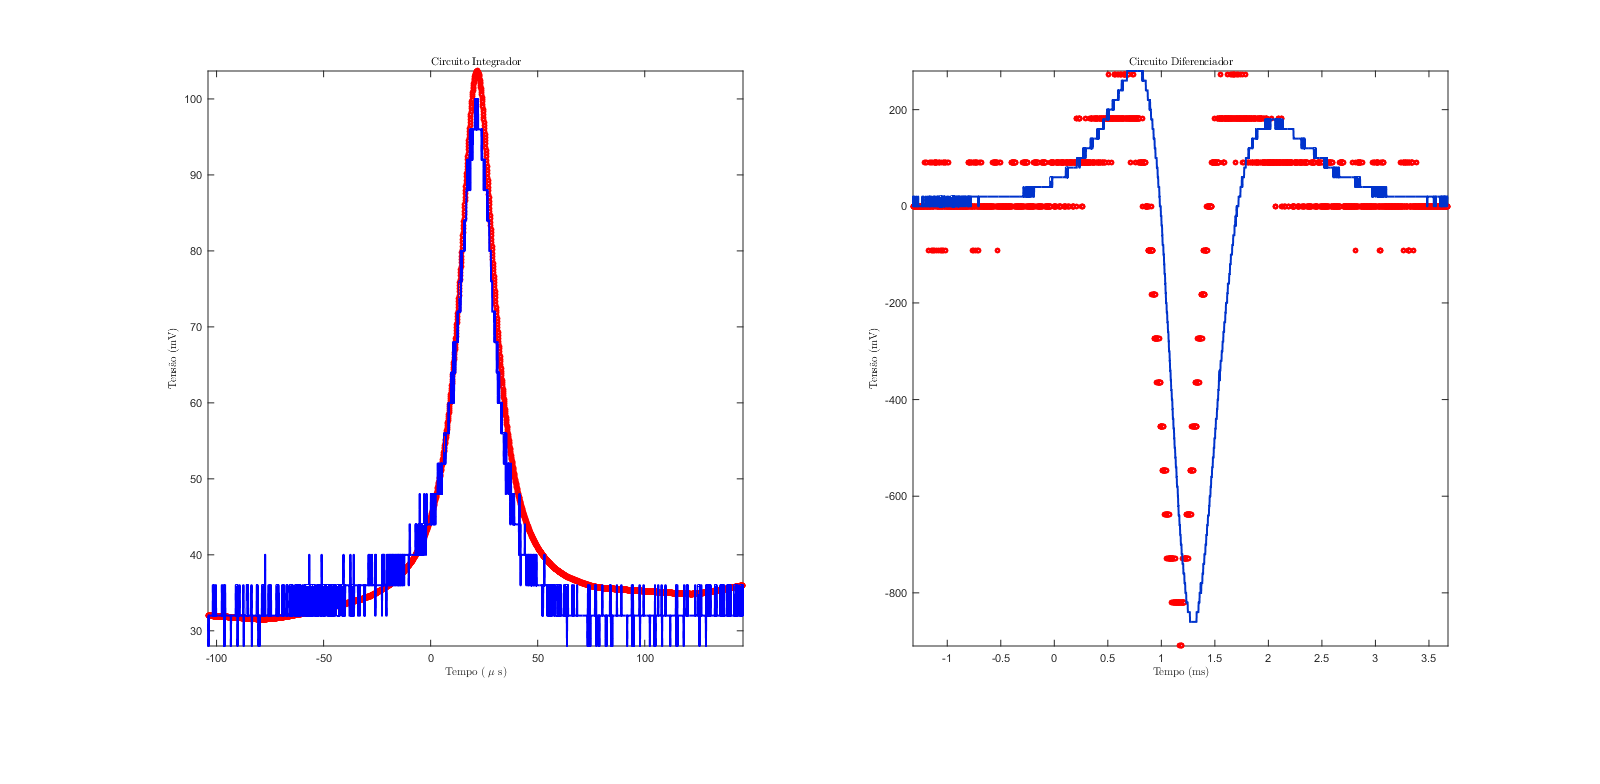
\includegraphics[scale=0.4]{Dlorentz.png}
        \caption{Curva da função \textit{Dlorentz} para os regimes de integração e diferenciação, respectivamente. O segundo gráfico apresenta os valores discretizados para a derivada numérica da curva com o erro associado.}
        \label{Dlorentz}
        \end{figure}
        
    Na \cref{Dlorentz}, pode-se observar que a curva da integração numérica corrigida, eliminando-se a componente DC, e a curva da derivação numérica correspondem às curvas esperadas. O comportamento corresponde ao esperado mesmo nos extremos da banda de frequência.
    
    
    \subsection{Transientes em circuitos RLC}
    
    
    Da parte B, temos a \cref{TransOscilo} e a \cref{CircuitoTriplo} que mostram o comportamento dos circuitos da \cref{CircResson} no transiente.
    Da \cref{eq:4}, é possível derivar os comportamentos esperados para cada um deles.
    
    
        \begin{figure}[!htb]
        \centering
        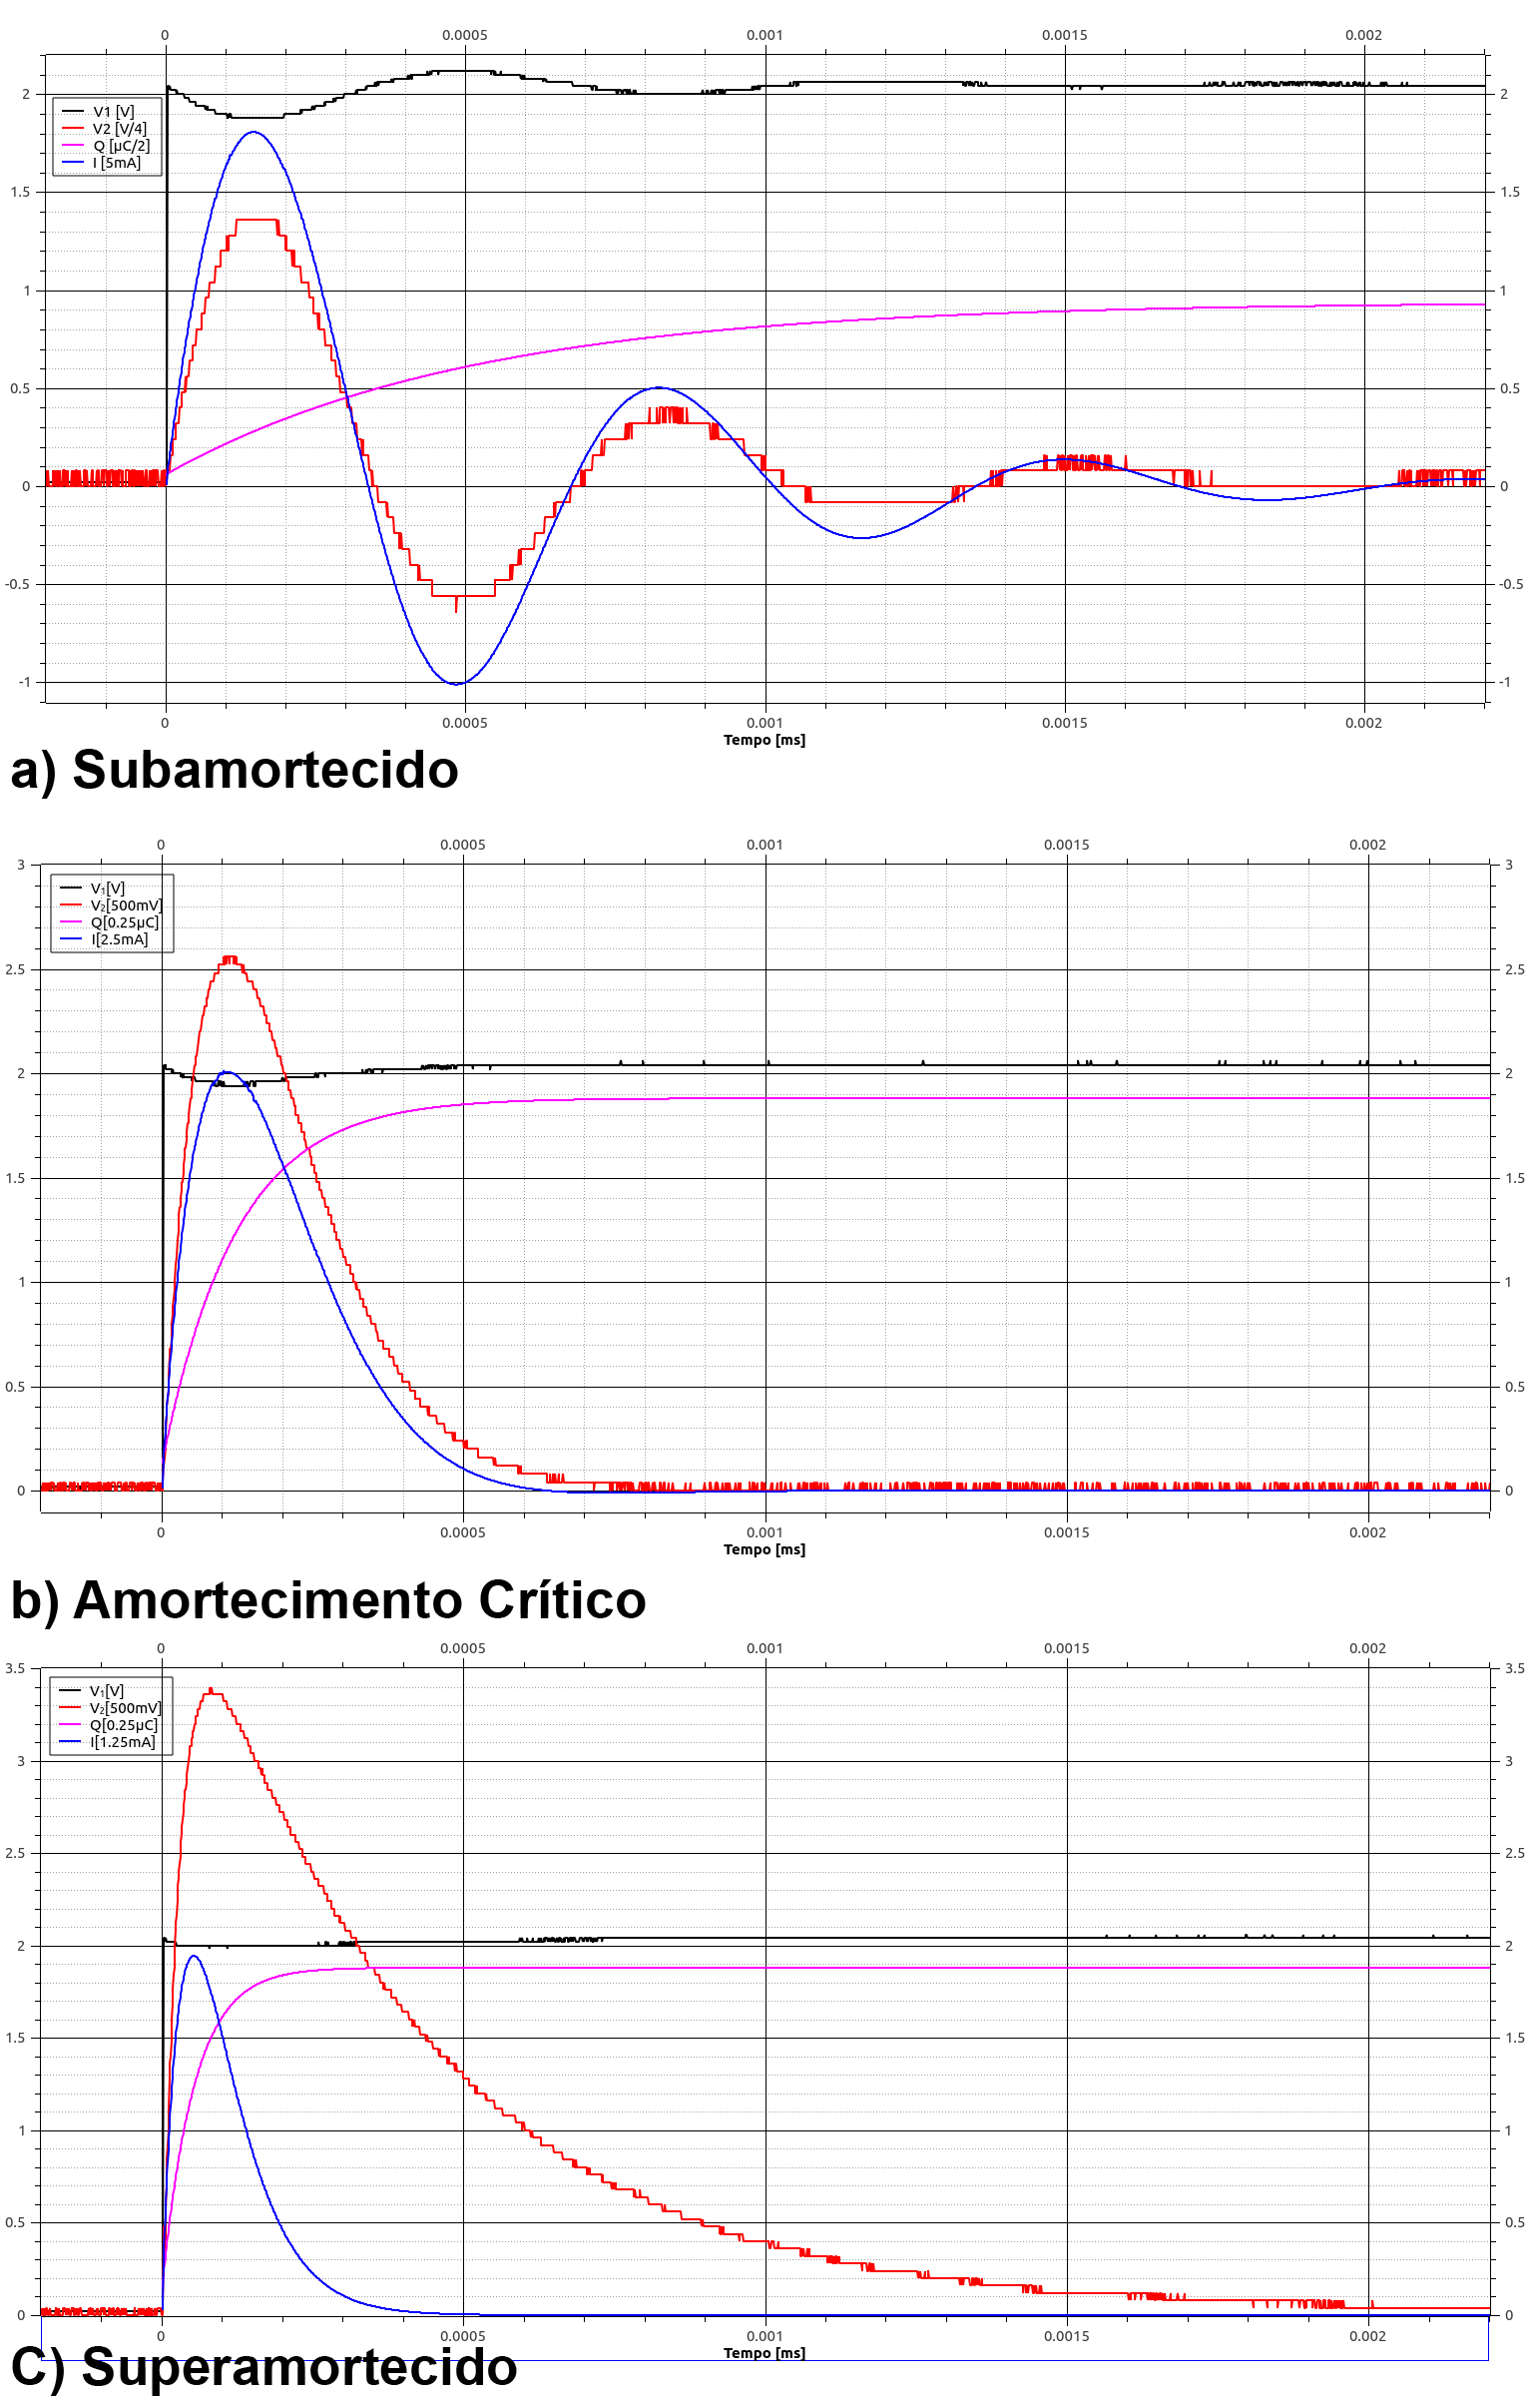
\includegraphics[scale=0.28]{Compara.png}
        \caption{gráficos das formas de onda observadas para os transientes dos circuitos RLC da \cref{CircResson} associados à forma de onda esperada gerada através das soluções da \cref{eq:2}.}
        \label{Compara}
        \end{figure}
    

    
    As imagens da \cref{Compara} mostram o comportamento obtido experimentalmente, comparado ao comportamento esperado pelas equações de solução da EDO da \cref{eq:4}.
    
        
    
    É possível notar que o comportamento obtido experimentalmente se assemelha muito ao que foi previsto pelas equações teóricas: as ondas possuem a mesma forma, e as variações de tamanho ou distância são mínimas.
    %provenientes dos erros do experimento, ou por diferenças nas escalas das curvas.
    
    
    Através do gráfico da \cref{Compara}a, do circuito subamortecido, é possível medir os intervalos dos máximos locais e estimar o período médio das oscilações. $T = (0.69 \pm 0.01) ms$. Com esse valor de período, obtém-se $\omega = {(91 \pm 1)10^2 \frac{rad}{s}}$, que tem a mesma ordem de grandeza da frequência angular de ressonância do circuito, medida com o osciloscópio observando-se a figura de Lissajous, $\omega _0 = (9356 \pm 6) \frac{rad}{s}$.Os dois valores são relativamente próximos, porém distintos. E esse fato não é surpresa, pois a freqüência de oscilação da resposta transiente difere naturalmente da frequência natural do circuito.
    
    
    Com esse mesmo gráfico, pode-se medir os pontos de máximos locais em módulo e plotar o gráfico da figura \cref{RetaLog}. Nele, a partir de regressão linear pode-se modelar o comportamento com a reta $y = (-18 \pm 2)100t + 0.4 \pm 0.2$. Nela, o coeficiente angular é o oposto do inverso da constante de tempo de oscilação da resposta transiente $\tau$. Onde $\tau = (0.55 \pm 0.03) {10^{-3}}{s}$.
    
    Para o circuito RLC, $\tau = \frac{2L}{R_D + R_G + R_L}$. Com os valores medidos de $R_D = (100 \pm 10)\Omega$, $R_G = (50.5 \pm 0.1)\Omega$ e $R_D = (46.5 \pm 0.1)\Omega$, calculamos $L = (54 \pm 4)mH$. 
    
    \begin{figure}[!htb]
    \centering
    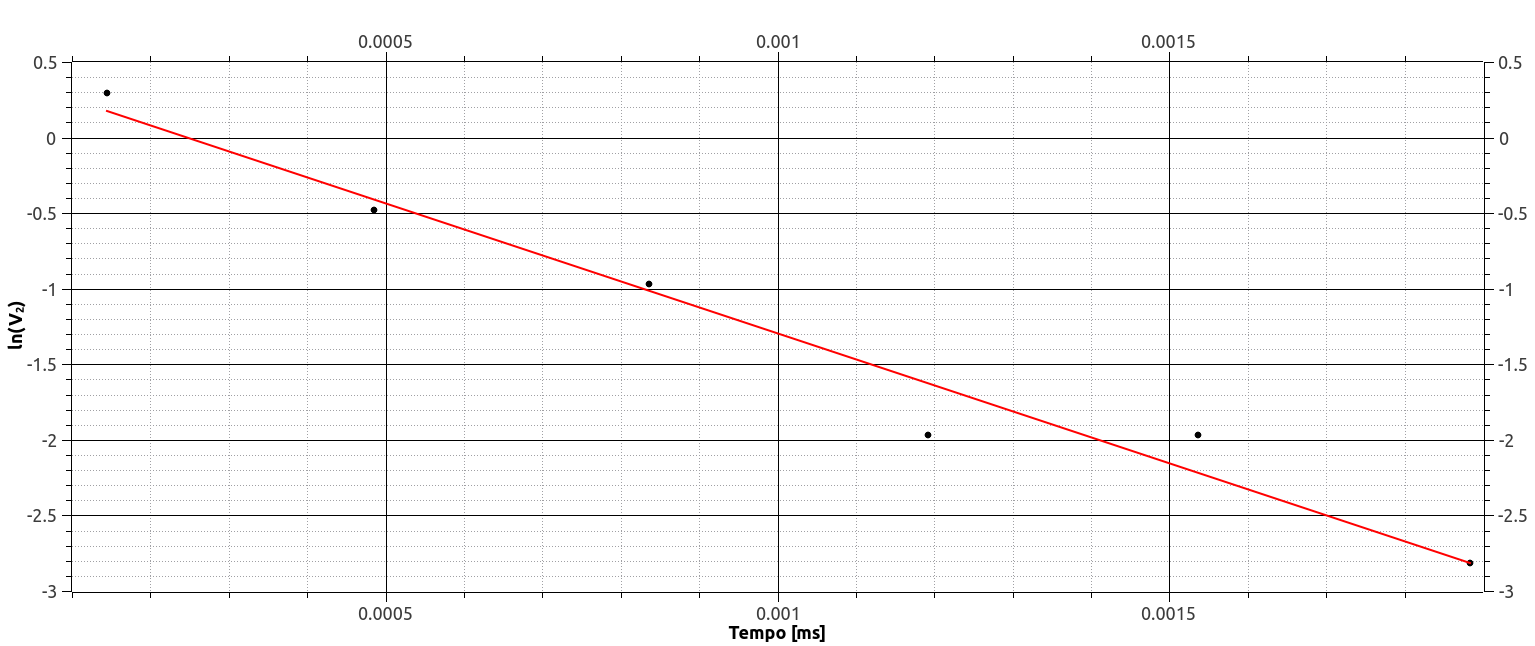
\includegraphics[scale=0.38]{RetaLog.png}
    \caption{Gráfico do logaritmo natural da tensão no resistor (ln($V_2$)) em relação ao tempo (em ms).}
    \label{RetaLog}
    \end{figure}
    
    
    No gráfico da \cref{SomaQuadrada}, pode-se observar que a onda da tensão de entrada e a onda da tensão no resistor têm forma semelhante, porém oposta. A onda vermelha, que representa a soma das duas é quadrada, o que prova que elas são complementares. Isso mostra que a queda de tensão da fonte devido à carga do circuito é proporcional à corrente, e proporcional à tensão medida no resistor. Isso é explicado considerando-se a resistência interna do gerador de funções, que não é nula.

\section{Discussão}

    Na parte A do experimento, foi possível estudar o comportamento dos circuitos passa-alta e passa-baixa em suas faixas de diferenciação e integração, respectivamente. Pudemos analisar como o comportamento de cada circuito muda quando a frequência é muito menor, próxima ou muito maior do que a sua frequência de corte, $f_0$.
    
    Observamos que, no caso do circuito passa-baixa, da \cref{CircIntegDif}b, a frequências baixas, é permitida a passagem de quase toda a tensão pelo circuito. A frequências muito mais altas do que $f_0$, é possível observar claramente o comportamento integrador do circuito, conforme representado na última linha da \cref{PassaBaixaVarredura}. Na função senoidal, observamos que as duas ondas em $V_1$ e $V_2$ são senoides, cuja diferença de fase, medida através do osciloscópio, é de $\phi$ =$(-89.20 \pm 0.01)^o$, o que é bem próximo do $-\pi /2$ esperado para a integral de uma função senoidal. Assim, foi possível averiguar que o circuito estava mesmo integrando as funções de entrada.
    
    Simetricamente, no caso do circuito passa-alta, \cref{CircIntegDif}a, pudemos observar que, a baixas frequências, ele atua como diferenciador, e com frequências altas toda a tensão de entrada é transmitida para a tensão de saída. Pudemos analisar a \cref{PassaAltaVarredura} e concluir que a diferença de fase nas ondas senoidais, em baixa frequência, também foi de $\pi /2$. Isso é o esperado da derivada de uma função senoidal.
    
    Ambos os casos podem ser observados ao analisar o comportamento da derivada e da integral da função \textit{Dlorentz}, que tiveram o comportamento esperado.
    
    Obtivemos, como valor da capacitância,  $C = 0.21 \pm 0.02 \mu F$, a qual está dentro do valor esperado ($C_0 = (0.22 \pm 0.02 \mu F)$).
    
    Da parte B do experimento, no estudo da solução homogênea da \cref{eq:4} e o comportamento dos circuitos ressonantes em transientes, foi possível notar que o comportamento obtido experimentalmente foi dentro do esperado pela literatura. Conforme a \cref{Compara}, que mostra as formas de onda obtidas com o osciloscópio para o comportamento do circuito e as curvas do resultado esperado através das soluções da \cref{eq:4}, os comportamentos estavam bem próximos e permitiram estudar o transiente nesse tipo de circuito ressonante.
    
    Com a variação do valor da resistência, através da resistência de década, foi possível observar o comportamento dos transientes nos casos subamortecido, amortecimento crítico e superamortecido, que também estavam dentro do esperado. No caso subamortecido, foi possível observar as oscilações durante o transiente da onda, e o resultado experimental bate com o proposto através das soluções da \cref{eq:4}, conforme pode ser observado na \cref{Compara}a, e o mesmo pode ser dito para os outros 2 estados de amortecimento.
    
    No gráfico da \cref{SomaQuadrada}, pudemos observar que a onda da tensão de entrada e a onda da tensão no resistor são complementares. Isso mostra que a queda de tensão da fonte devido à carga do circuito é proporcional à corrente, e proporcional à tensão medida no resistor. Isso se deve pois a resistência interna do gerador de funções não é nula.
    
    As principais fontes de erro são os erros instrumentais, a resistência interna dos cabos e a dificuldade de um encaixe perfeito usando a \textit{Protoboard} e os equipamentos adaptados disponíveis.
    
    
\section{Conclusão}

    Através dos resultados obtidos no experimento, é possível concluir que ele estava dentro do esperado pela literatura. O comportamento dos circuitos RC na primeira parte, como circuitos integradores e diferenciadores, seguiu o proposto pela integração ou diferenciação das funções de entrada, conforme foi possível observar na faixa de alta frequência para o circuito passa-baixa e na faixa de baixa frequência para o circuito passa-alta, respectivamente o comportamento integrador e diferenciador do circuito.
    
    A capacitância do circuito calculada através dos dados obtidos experimentalmente foi de $C=0.21\pm 0.02 \mu F$, que está dentro do valor esperado do capacitor utilizado que tinha Capacitância nominal de $C=0.22\pm 0.02 \mu F$.
    
    A forma do transiente estudada para os circuitos RLC, também estava dentro do esperado conforma a literatura descrita. As curvas obtidas para as três situações de amortecimento (subamortecimento, amortecimento crítico e superamortecido) foram condizentes, seguiu o proposto pelas soluções da \cref{eq:4}, como pode ser observado na \cref{Compara}.
    
    A frequência de oscilação da resposta transiente encontrada foi de $\omega = (91 \pm 1)10^2 \frac{rad}{s}$ e a frequência natural de oscilação obtida através da análise das figuras de \textit{Lissajous} foi de $\omega _0 = (9356 \pm 6)\frac{rad}{s}$, e a constante de tempo para o circuito montado pode ser calculada como sendo $\tau = (0.55 \pm 0.03)10^{-3}s$.

\section{Instrumentos utilizados}
Os instrumentos utilizados neste experimento foram,
\begin{itemize}
	\item Osciloscópio Tektronix 10002B
	\item Gerador de funções arbitrárias BK Instruments 4052
	\item Multímetro DT830 Digital
\end{itemize}


\section{Propagação de erros \label{ap:erros}}

\begin{enumerate}
    \item Erro da frequência de corte $f_0$ calculada através de \cref{f0}: \\$\Delta f_{0}=\dfrac {1}{4\pi ^{2}R^{2}C^{2}}\left( \dfrac {\Delta R^{2}}{R^{2}}+\dfrac {\Delta c^{2}}{c^{2}}\right)$
    \item Erro da Capacitância C calculada através da \cref{eq:2}\\
    $\Delta C^{2}=\dfrac {1}{\left( V_{2}2\pi FR\right) ^{2}}(\Delta V^{2}_{1}+\Delta V^{2}_{2}\left( \dfrac {V_{1}}{V_{2}}\right) ^{2}+\Delta F^{2}\left( \dfrac {V_{1}}{F}\right) ^{2}+\Delta R^{2}\left( \dfrac {V_{1}}{R}\right) ^{2}$
    \item Erro da frequência angular $\omega :$\\
    $\Delta \omega^{2}=\dfrac {4\pi^2}{(T^4)(\Delta T)^2}$
    \item Erro da frequência natural $\omega _0:$\\
    $\Delta \omega_0 = {2\pi}{\Delta f}$
    \item Erro da constante de tempo $\tau:$\\
    $\Delta \tau = \frac{\Delta A}{2A^2}$
    \item Erro da indutância $L:$\\
    $\Delta L^2 = \frac{(R_D + R_G + R_L)^2 (\Delta \tau)^2}{4} + \frac{\tau ^2(\Delta R_D)^2}{4} + \frac{\tau ^2(\Delta R_G)^2}{4} + \frac{\tau ^2(\Delta R_L)^2}{4}$
\end{enumerate}


\newpage
\begin{thebibliography}{10}

\bibitem{apostila}Gustavo Wiederhecker e colaboradores, \textsl{Roteiros de F429 - Corrente alternada e óptica.} Compilado em 26 de setembro de 2016.

\bibitem{livro texto}[Boyce and DiPrima, 2009 Boyce, W. E. and DiPrima, R. C. (2009)]. Elementary differential equations and boundary value problems. Wiley, Hoboken, NJ, 9th ed edition.

\bibitem{livro}[Yaro Burian Jr. e Ana Cristina Lyra]. Circuitos Elétricos.

\end{thebibliography}

\end{document}